\documentclass[11pt]{article}

% ---------- Typography ----------
\usepackage{lmodern}
\usepackage[T1]{fontenc}
\usepackage[utf8]{inputenc}
\usepackage{cmap}
\input{glyphtounicode}
\pdfgentounicode=1
\usepackage[final,expansion=false,protrusion=true]{microtype}
\usepackage[a4paper,top=2.6cm,bottom=2.6cm,left=2.8cm,right=2.8cm]{geometry}
\linespread{1.05}
\widowpenalty=10000 \clubpenalty=10000
\emergencystretch=2em

% ---------- Mathematics ----------
\usepackage{amsmath,amssymb,amsthm,mathtools}
\usepackage{booktabs,array,enumitem}
\usepackage[dvipsnames]{xcolor}
\usepackage{tikz}
\usepackage{pgfplots}
\usepackage{placeins}
\pgfplotsset{compat=1.18}
\usepgfplotslibrary{groupplots}
\usetikzlibrary{arrows.meta,positioning,calc}
\usepackage[colorlinks=true,linkcolor=NavyBlue,citecolor=NavyBlue,urlcolor=NavyBlue]{hyperref}
\hypersetup{
  pdftitle={Anatomy of a Cohomology Wall: the Koszul section-map rank defect on the tetraquadric Calabi-Yau threefold},
  pdfauthor={Santiago Maniches},
  pdfsubject={Algebraic geometry; line-bundle cohomology on Calabi-Yau threefolds},
  pdfkeywords={cohomology wall, line bundle cohomology, tetraquadric, Calabi-Yau threefold, Koszul complex, Fitting ideal, Buchsbaum-Rim, Thom-Porteous, determinantal degeneracy locus}
}

% ---------- Theorem environments ----------
\theoremstyle{plain}
\newtheorem{theorem}{Theorem}[section]
\newtheorem{proposition}[theorem]{Proposition}
\newtheorem{lemma}[theorem]{Lemma}
\newtheorem{corollary}[theorem]{Corollary}
\newtheorem{conjecture}[theorem]{Conjecture}
\theoremstyle{definition}
\newtheorem{definition}[theorem]{Definition}
\theoremstyle{remark}
\newtheorem{remark}[theorem]{Remark}

% ---------- Claim-discipline macros ----------
\newcommand{\Proven}{\textcolor{ForestGreen}{\textsf{[proven]}}}
\newcommand{\Computed}{\textcolor{Sepia}{\textsf{[computed]}}}
\newcommand{\Open}{\textcolor{BrickRed}{\textsf{[open]}}}

% ---------- Notation ----------
\newcommand{\PP}{\mathbb{P}}
\newcommand{\cO}{\mathcal{O}}
\newcommand{\cI}{\mathcal{I}}
\newcommand{\cC}{\mathcal{C}}
\newcommand{\cZ}{\mathcal{Z}}
\newcommand{\rank}{\operatorname{rank}}
\newcommand{\defect}{\operatorname{def}}
\DeclareMathOperator{\Coker}{coker}
\DeclareMathOperator{\Ker}{ker}
\DeclareMathOperator{\Bs}{Bs}

\title{\textbf{Anatomy of a Cohomology Wall}\\[2pt]
\large The Koszul section-map rank defect on the tetraquadric Calabi--Yau threefold}
\author{Santiago Maniches\thanks{ORCID: 0009-0005-6480-1987. Contact: \texttt{santiago.maniches@proton.me}.}\\
\small Independent researcher}
\date{6 July 2026}

\begin{document}
\maketitle

\begin{abstract}
\noindent
Line-bundle cohomology on Calabi--Yau threefolds is piecewise polynomial in the line-bundle charges, with the polynomial pieces separated by walls~\cite{ConstantinLukas2019}; the values are computable by established tools~\cite{cohomCalg}, and proofs of such formulae exist for surfaces and certain threefolds via vanishing-theorem and Zariski-chamber techniques~\cite{BCDL2020,BC2020}. This note dissects the \emph{mechanism} of one wall family on the tetraquadric $X=[(\PP^1)^4\,\|\,(2,2,2,2)]$, for charges $D=(-a_1,-a_2,-a_3,b)$ with $a_i\ge 4$ and $b\ge 2$.

We prove a closed-form rank formula for the Koszul connecting map at $b=2$, and we prove that the rank defect saturates at the constant $48=3!\cdot 2^3$ for all $a_i\ge 6$, by two independent arguments: a finite-difference identity on the Koszul complex, and an identification of the cokernel with the cohomology of a base-locus scheme of degree $\deg\mathcal{Z}=\int_Y c_1(\mathcal{O}(2,2,2))^3=48$. The wall structure reflects two distinct piecewise phenomena: boundary $H^1$ corrections that activate where individual ambient $H^1$ groups switch on, and a separate source-target minimum flip. The rank formula is verified against $22$ independently computed charge vectors ($22/22$ exact).

For $b\ge 3$ the section map reduces to a genuinely partial contraction. We prove a general Toeplitz determinantal theorem for every $b\ge2$: the maximal-minor ideal of the section-induced Toeplitz map is exactly the $(b-1)$st power of the length-$48$ base-locus ideal, the local cokernel has length $48\binom{b+1}{3}$, and in the acyclic range $a_i\ge2b+1$ the global rank defect is given by an explicit source-target formula. The Thom--Porteous ceiling occurs precisely when $(b+1)\prod_i(a_i-1)\ge(b-1)\prod_i(a_i+1)$. Exact finite-field computations at $b=4$ and $b=5$ become verification data for this theorem and rule out the competing factorial pattern.
\end{abstract}

\section{Setup}\label{sec:setup}

The tetraquadric $X=[(\PP^1)^4\,\|\,(2,2,2,2)]$ is the smooth zero locus of a generic section $s\in H^0(A,\cO_A(N))$ of $N=(2,2,2,2)$ on the ambient space $A=(\PP^1)^4$. It is a Calabi--Yau threefold with $(h^{1,1},h^{2,1})=(4,68)$, $\chi=-128$. For a line bundle $L=\cO_X(D)$, $D\in\mathbb{Z}^4$, cohomology is computed from the Koszul sequence
\begin{equation}\label{eq:koszul}
0\longrightarrow \cO_A(D-N)\xrightarrow{\;\cdot s\;}\cO_A(D)\longrightarrow \cO_X(D)\longrightarrow 0 .
\end{equation}
Ambient groups factor through K\"unneth from the $\PP^1$ atoms,
\begin{equation}\label{eq:p1}
h^0(\PP^1,\cO(k))=\max(k+1,0),\qquad
h^1(\PP^1,\cO(k))=\max(-k-1,0).
\end{equation}
The long exact sequence of~\eqref{eq:koszul} contains the connecting multiplication map
\begin{equation}\label{eq:alpha}
\alpha:\;H^q\!\big(A,\cO_A(D-N)\big)\longrightarrow H^q\!\big(A,\cO_A(D)\big),
\end{equation}
in the degree $q$ where both groups are nonzero (the \emph{section regime}).

\begin{definition}[Rank defect]
$\defect(D):=\min\!\big(\dim_{\mathrm{src}},\dim_{\mathrm{tgt}}\big)-\rank\alpha\;\ge 0$, where src and tgt are the source and target of~\eqref{eq:alpha}. A bundle is \emph{defective} when $\defect(D)>0$.
\end{definition}

\section{The family and the contraction mechanism}\label{sec:mech}

Fix the sign pattern with three negative charges,
\[
D=(-a_1,-a_2,-a_3,\,b),\qquad a_i\ge 4,\;\; b\ge 2,
\]
so that $q=3$ in~\eqref{eq:alpha}: the three negative factors carry $H^1$, the fourth carries $H^0$. Write $a=(a_1,a_2,a_3)$ and let $Y=(\PP^1)^3$ carry the unnamed cohomology below.

\begin{figure}[t]
\centering
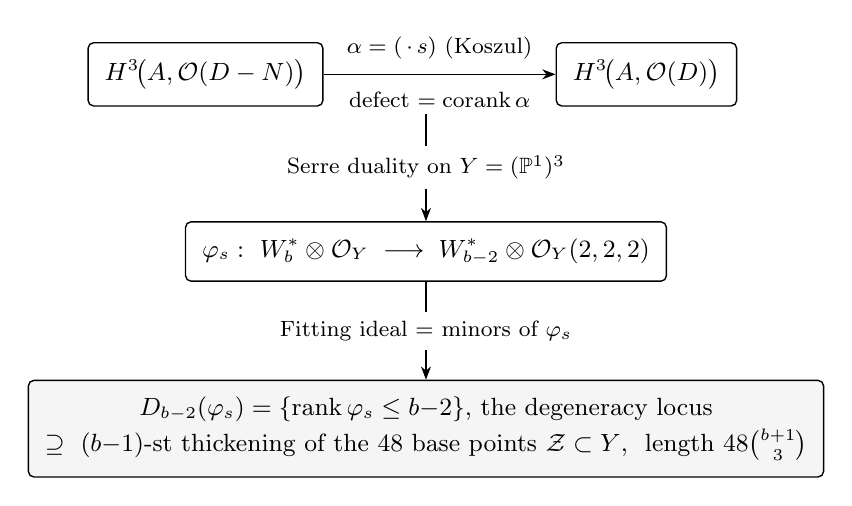
\begin{tikzpicture}[
  >=Stealth,
  box/.style={draw, rounded corners=2pt, align=center, inner sep=6pt, line width=0.5pt, font=\small}
]
\node[box] (src) at (-3.3,0) {$H^3\!\big(A,\cO(D-N)\big)$};
\node[box] (tgt) at ( 2.3,0) {$H^3\!\big(A,\cO(D)\big)$};
\draw[->] (src) -- node[above=2pt, font=\footnotesize]{$\alpha=(\,\cdot\, s)$\ (Koszul)}
                   node[below=3pt, font=\footnotesize]{defect $=\operatorname{corank}\alpha$} (tgt);
\node[box] (phi) at (-0.5,-2.25) {$\varphi_s:\ W_b^{*}\otimes\cO_Y \;\longrightarrow\; W_{b-2}^{*}\otimes\cO_Y(2,2,2)$};
\draw[->] (-0.5,-0.5) -- (phi.north)
   node[midway, fill=white, font=\footnotesize]{Serre duality on $Y=(\PP^1)^3$};
\node[box, fill=black!4] (deg) at (-0.5,-4.5) {$D_{b-2}(\varphi_s)=\{\rank\varphi_s\le b{-}2\}$, the degeneracy locus\\[2pt]
   $\supseteq\ (b{-}1)$-st thickening of the $48$ base points $\cZ\subset Y$,\ \ length $48\tbinom{b+1}{3}$};
\draw[->] (phi.south) -- (deg.north)
   node[midway, fill=white, font=\footnotesize]{Fitting ideal $=$ minors of $\varphi_s$};
\end{tikzpicture}
\caption{The mechanism in one picture. The connecting Koszul section map $\alpha$ on the ambient $A=(\PP^1)^4$ dualises, by Serre duality on $Y=(\PP^1)^3$, to a contraction $\varphi_s$ of vector bundles of ranks $(b{+}1)\to(b{-}1)$. The section-induced Toeplitz form is now computed exactly for every $b\ge2$: its maximal-minor ideal is the $(b{-}1)$st power of the $48$-point base-locus ideal, and its local cokernel length is $48\binom{b+1}{3}$ (Theorem~\ref{thm:general-toeplitz-saturation}). After twisting in the acyclic range, the global defect is governed by the same length together with the source-target minimum.}
\label{fig:mechanism}
\end{figure}

\begin{proposition}[Reduction; explicit dimensions]\label{prop:reduction}
\Proven\ Set $W_k=H^0(\PP^1,\cO(k))$. By K\"unneth and~\eqref{eq:p1},
\[
\dim_{\mathrm{src}}=h^3(A,\cO(D-N))=(b-1)\prod_{i=1}^3(a_i+1),
\qquad
\dim_{\mathrm{tgt}}=h^3(A,\cO(D))=(b+1)\prod_{i=1}^3(a_i-1).
\]
Serre duality on $A$ (with $K_A=\cO(-2,-2,-2,-2)$), under which multiplication by $s$ is self-adjoint, identifies $\rank\alpha$ with the rank of the partial contraction
\begin{equation}\label{eq:partial}
\widetilde{\mu}:\;H^0\big(Y,\cO(a-2)\big)\otimes W_b^{\;*}\longrightarrow H^0\big(Y,\cO(a)\big)\otimes W_{b-2}^{\;*},
\end{equation}
where $s=\sum_m s_m\otimes y^m$ ($y^m$ a monomial basis of $W_b$, slices $s_m\in H^0(Y,\cO(2,2,2))$) acts by $\xi\otimes\lambda\mapsto\sum_m (s_m\xi)\otimes(\lambda\,\lrcorner\, y^m)$. For $b=2$ the residual factor $W_0^{\,*}$ is trivial and~\eqref{eq:partial} collapses to the multiplication map
\begin{equation}\label{eq:mult}
\mu:\;U\otimes H^0\big(\cO(a-2)\big)\longrightarrow H^0\big(\cO(a)\big),
\qquad U=\langle s_1,s_2,s_3\rangle\subset H^0\big(\cO(2,2,2)\big).
\end{equation}
\end{proposition}

\begin{proof}
The K\"unneth dimensions follow from~\eqref{eq:p1}: for $\cO(D)$ the unique degree-$3$ contribution takes $H^1$ on the three negative factors ($\dim a_i-1$) and $H^0(\cO(b))$ ($\dim b+1$); for $\cO(D-N)$ the same with $-a_i-2$ ($\dim a_i+1$) and $\cO(b-2)$ ($\dim b-1$). Dualizing $\alpha$ and applying Serre duality factorwise, $H^1(\PP^1,\cO(k))^*\cong H^0(\PP^1,\cO(-k-2))$, turns each negative factor's $H^1$ into polynomial spaces and the fourth factor's $H^0(\cO(b))$, $H^0(\cO(b-2))$ into their duals; multiplication by $s$ becomes the stated contraction. Self-adjointness of multiplication under the Serre pairing gives $\rank\alpha=\rank\widetilde{\mu}$.
\end{proof}

\begin{proposition}[Dichotomy]\label{prop:dichotomy}
For generic $s$:
\begin{enumerate}[leftmargin=2.2em,itemsep=2pt]
\item \Proven\ \textbf{$b=2$.} $U$ is spanned by a regular sequence (Lemma~\ref{lem:slices}); its base scheme $\cZ\subset Y$ is finite of length $\deg\cZ=\int_Y(2H_1+2H_2+2H_3)^3=3!\cdot 2^3=48$.
\item \Proven\ \textbf{General $b\ge2$ Toeplitz saturation in the acyclic range.} The reduction is the genuinely partial contraction~\eqref{eq:partial}. The section-induced Toeplitz maximal-minor ideal and the Buchsbaum--Rim cokernel length are computed for all $b\ge2$, and for $a_i\ge2b+1$ the global defect is the piecewise source-target formula of Theorem~\ref{thm:general-toeplitz-saturation}.
\item \Proven\ \textbf{$2{+}2$ pattern $(-a_1,-a_2,b_1,b_2)$.} For $b_1=b_2=2$, the contraction is multiplication by the $9$-dimensional linear system $V\subset H^0\big((\PP^1)^2,\cO(2,2)\big)$ cut out by the slices of $s$. Since $\cO(2,2)$ is very ample on $(\PP^1)^2$ and three generic sections of a very ample bundle on a surface already have empty common zero locus (expected codimension $3>2$), the base scheme of $V$ is empty~\cite[III.10.9]{Hartshorne}. Emptiness alone gives only surjectivity of the \emph{sheaf} map; surjectivity on $H^0$ (hence $\defect=0$) follows because the kernel sheaf, resolved by the Koszul complex of the slices, has vanishing $H^1$: on the surface $(\PP^1)^2$ every relevant twist $a-2,a-4$ has non-negative entries for $a_i\ge 4$, so $H^1=0$ by K\"unneth (the same non-negativity as in Proof~2 of Theorem~\ref{thm:ceiling}, with one fewer Koszul step). Thus $\defect=0$ for all $a_i\ge 4$.
\end{enumerate}
\end{proposition}

\section{The rank formula at \texorpdfstring{$b=2$}{b=2}: a complete proof}\label{sec:b2}

\begin{lemma}[Slices of a generic section]\label{lem:slices}
\Proven\ Let $V=H^0(Y,\cO(2,2,2))$ and $W=H^0(\PP^1,\cO(2))$.
\begin{enumerate}[leftmargin=2.2em,itemsep=2pt]
\item The slice map $H^0(A,\cO(2,2,2,2))\cong V\otimes W\to V^{\oplus 3}$, $s\mapsto(s_1,s_2,s_3)$, is a linear isomorphism.
\item For $(s_1,s_2,s_3)$ in a dense Zariski-open subset of $V^{\oplus 3}$, the common zero scheme $\cZ=Z(s_1,s_2,s_3)\subset Y$ is finite, and $\dim\langle s_1,s_2,s_3\rangle=3$.
\item For such triples, $(s_1,s_2,s_3)$ is a regular sequence on $Y$; the Koszul complex
\begin{equation}\label{eq:koszulres}
0\to\cO(a-6)\to\cO(a-4)^{\oplus 3}\to\cO(a-2)^{\oplus 3}\xrightarrow{\;\mu\;}\cO(a)\to\cO_{\cZ}(a)\to 0
\end{equation}
is exact, and $\deg\cZ=48$.
\end{enumerate}
Consequently, the slices of a \emph{generic} $s\in H^0(A,\cO(2,2,2,2))$ satisfy (2)--(3).
\end{lemma}

\begin{proof}
(1) is K\"unneth plus the choice of a monomial basis of $W$: the coordinates of $s\in V\otimes W$ in that basis \emph{are} the slices, and $\dim(V\otimes W)=27\cdot 3=\dim V^{\oplus 3}$.
(2) $\cO(2,2,2)$ is very ample on the smooth projective threefold $Y$; embed $Y\subset\PP^{26}$ by $|V|$. By Bertini (char.~$0$)~\cite[II.8.18, III.7.9.1]{Hartshorne}, a generic member of $|V|$ is a smooth surface, a generic second section cuts it in a smooth curve, and a generic third meets that curve in a finite scheme; linear independence of a generic triple is clear. The locus of triples with $\dim Z\ge 1$ is Zariski-closed (upper semicontinuity of fiber dimension on the incidence variety), so its complement is the required dense open set.
(3) $Y$ is smooth, hence Cohen--Macaulay. At points of $\cZ$ the three local equations cut a codimension-$3$ subscheme of a $3$-dimensional CM local ring, hence form a regular sequence; away from $\cZ$ some $s_i$ is a unit. Exactness of the Koszul complex on a regular sequence is standard~\cite[Cor.~17.5]{Eisenbud}. Properness of the intersection gives B\'ezout on $Y$: $\deg\cZ=\int_Y c_1(\cO(2,2,2))^3=3!\cdot 2^3=48$. For generic $s$ the three divisors meet transversally, so $\cZ$ is reduced: $48$ distinct points, each a complete-intersection point with regular local ring (this is the reducedness used in Theorem~\ref{thm:general-toeplitz-saturation} for the local length count). By (1), generic $s$ yields a generic triple.
\end{proof}

\begin{theorem}[Rank formula, $b=2$]\label{thm:rank}
\Proven\ Let $D=(-a_1,-a_2,-a_3,2)$, $a_i\ge 4$, $s$ generic. With all cohomology on $Y$ and the convention~\eqref{eq:p1} extended by K\"unneth,
\begin{equation}\label{eq:rankformula}
\rank\alpha \;=\; 3\prod_{i=1}^{3}(a_i-1)\;-\;\Big[\,3\,h^0(a-4)\;-\;h^0(a-6)\;+\;h^1(a-6)\,\Big],
\end{equation}
\begin{equation}\label{eq:defectformula}
\defect(D)\;=\;\min\!\Big(\textstyle\prod_i(a_i+1),\;3\prod_i(a_i-1)\Big)\;-\;\rank\alpha .
\end{equation}
\end{theorem}

\begin{proof}
By Proposition~\ref{prop:reduction}, $\rank\alpha=\rank\mu$ with $\mu$ as in~\eqref{eq:mult}, a map from a space of dimension $3\,h^0(a-2)=3\prod(a_i-1)$. By left-exactness of $H^0$, $\Ker\mu=H^0(K_2)$ for the kernel sheaf $K_2=\Ker\big(\cO(a-2)^{\oplus3}\to\cO(a)\big)$, which by Lemma~\ref{lem:slices}(3) sits in
\[
0\to\cO(a-6)\to\cO(a-4)^{\oplus 3}\to K_2\to 0 .
\]
Its long exact sequence gives
\[
h^0(K_2)=3h^0(a-4)-h^0(a-6)+\dim\Ker\!\Big(H^1(\cO(a-6))\to H^1\big(\cO(a-4)^{\oplus3}\big)\Big).
\]
The decisive vanishing: for $a_i\ge 4$ every entry of $a-4$ is non-negative, so by K\"unneth and~\eqref{eq:p1}, $H^1\big(Y,\cO(a-4)\big)=0$ \emph{identically on the domain}. Hence the kernel above is all of $H^1(\cO(a-6))$, of dimension $h^1(a-6)$, and $h^0(K_2)$ equals the bracket in~\eqref{eq:rankformula}. Then $\rank\mu=3\prod(a_i-1)-h^0(K_2)$, which is~\eqref{eq:rankformula}; and~\eqref{eq:defectformula} is the definition of $\defect$ with the dimensions of Proposition~\ref{prop:reduction} at $b=2$.
\end{proof}

\begin{remark}[The minimum flips]\label{rem:minflip}
\Proven\ $\mathrm{src}=\prod(a_i+1)$ and $\mathrm{tgt}=3\prod(a_i-1)$ satisfy $\mathrm{tgt}<\mathrm{src}$ on the low boundary (e.g.\ $(4,4,4)$: $81<125$) but $\mathrm{src}<\mathrm{tgt}$ for all $a_i\ge 6$, since $\prod_i\frac{a_i+1}{a_i-1}\le(7/5)^3=\frac{343}{375}\cdot 3<3$. The defect is insensitive to the flip (Theorem~\ref{thm:ceiling}); the formula~\eqref{eq:defectformula} handles both regimes uniformly.
\end{remark}

\begin{remark}[The walls]\label{rem:walls}
\Proven\ The defect~\eqref{eq:defectformula} has two distinct sources of piecewise behaviour. First, the $h^1$ correction terms in the rank formula~\eqref{eq:rankformula} switch on precisely where an entry of $a-6$ crosses $-2$, i.e.\ where a single ambient $H^1$ activates; on the domain $a_i\ge4$ this happens exactly at entries $a_i=4$. At $a=(4,6,6)$, $h^1(\cO(-2,0,0))=1$ contributes $\defect=28=27+1$, falsifying any single global cubic. Second, $\defect=\min(\dim_{\mathrm{src}},\dim_{\mathrm{tgt}})-\operatorname{rank}$ carries the factor $\min(\dim_{\mathrm{src}},\dim_{\mathrm{tgt}})$, and which argument is smaller flips with the charges (for equal $a_i$ the minimum is $\dim_{\mathrm{tgt}}$ at $a_i\le5$ and $\dim_{\mathrm{src}}$ at $a_i\ge6$); this source-target flip is a separate saturation effect, not an $H^1$ wall.
\end{remark}

\section{The ceiling: two proofs}\label{sec:ceiling}

\begin{theorem}[Saturation ceiling]\label{thm:ceiling}
\Proven\ For all $a_i\ge 6$, $\defect(D)=48$.
\end{theorem}

\begin{proof}[Proof 1 (finite-difference identity)]
For $a_i\ge 6$ every entry of $a-6$ is non-negative, so $h^1(a-6)=0$, and by Remark~\ref{rem:minflip} the minimum is $\mathrm{src}=\prod(a_i+1)$. Define the cubic polynomial $f(t)=\prod_{i=1}^3(a_i+1-2t)$, so that
\[
f(0)=\textstyle\prod(a_i+1),\quad f(1)=\prod(a_i-1),\quad f(2)=h^0(a-4),\quad f(3)=h^0(a-6).
\]
Then by Theorem~\ref{thm:rank},
\[
\defect = f(0)-3f(1)+3f(2)-f(3) = -\Delta^3 f(0)
= -\,3!\cdot(\text{lead.\ coeff.\ of }f) = -\,6\cdot(-2)^3 = 48,
\]
since the third finite difference of a cubic is constant. This holds identically in $(a_1,a_2,a_3)$.
\end{proof}

\begin{proof}[Proof 2 (geometric: the base locus)]
For $a_i\ge 6$ all twists $a-2,a-4,a-6$ in~\eqref{eq:koszulres} have non-negative entries, so all their higher cohomology on $Y$ vanishes (K\"unneth). Chasing the two short exact sequences built from~\eqref{eq:koszulres}: $H^1(K_2)$ is squeezed between $H^1(\cO(a-4)^{\oplus3})=0$ and $H^2(\cO(a-6))=0$, hence vanishes, so $H^0(\cO(a-2)^{\oplus3})\twoheadrightarrow H^0(\cI_{\cZ}(a))$, i.e.\ $\operatorname{im}\mu=H^0(\cI_\cZ(a))$; and $H^1(\cI_\cZ(a))$ is squeezed between $H^1(\cO(a-2)^{\oplus3})=0$ and $H^2(K_2)=0$, hence vanishes, so $H^0(\cO(a))\twoheadrightarrow H^0(\cO_\cZ(a))$. Therefore
\[
\Coker\mu\;\cong\;H^0(\cO_{\cZ}(a))\;\cong\;k^{48},
\]
the length of the base scheme (Lemma~\ref{lem:slices}). The defect equals this cokernel dimension in the saturated regime, independent of the charges: a genuine infinite ceiling.
\end{proof}

\begin{remark}[Why $3!\cdot 2^3$]\label{rem:why48}
\Proven\ Proof~1 explains the numerology: the $3!$ is the third finite difference (three Koszul steps on a threefold), the $2^3$ is the cube of the step ($N$ shifts charges by $2$). Proof~2 identifies the same number as $\deg\cZ=\int_Y(2H_1+2H_2+2H_3)^3$. The agreement of the combinatorial and geometric counts is the content of the saturation.
\end{remark}

\section{Higher fourth charge: the partial contraction and a decisive test}\label{sec:bgen}

For $b\ge 3$ the reduction~\eqref{eq:partial} does not collapse to a single multiplication map: the residual factor $W_{b-2}^{\,*}$ has dimension $b-1\ge 2$. Computation at $b=3$ (and spot checks at $b=4$) shows the defect is governed, between the walls, by the cubic interior law
\begin{equation}\label{eq:blaw}
\defect(D)\;=\;(b+1)\prod_{i=1}^{3}\big(a_i-(2b-1)\big)
\end{equation}
between the walls, with small boundary $h^1$ corrections of the same type as Remark~\ref{rem:walls} (e.g.\ $(-6,-8,-8,3)\mapsto 38=36+2$, and $(-8,-8,-8,3)\mapsto 106=108-2$), and a deep-region constant ceiling: $192$ at $b=3$, first attained at $(9,9,9)$ and stable above it (also at $(10,10,10)$, $(8,9,10)$), while below it the defect is strictly sub-ceiling --- the equal-charge ladder reads $4,32,106$ at $a_i=6,7,8$. The corrected ceiling criterion is proved below in Theorem~\ref{thm:general-toeplitz-saturation}.


\subsection{The general Toeplitz saturation theorem}\label{sec:general-saturation}

The finite-field computations above are explained by a stronger structural statement.  The special section-induced map is not merely expected to have the Thom--Porteous length.  Its Toeplitz maximal-minor ideal can be computed exactly for every $b\ge2$, and the global rank defect is then determined by the source-target dimensions once the Buchsbaum--Rim resolution is acyclic.

\begin{theorem}[General Toeplitz determinantal saturation]\label{thm:general-toeplitz-saturation}
\Proven\ Let $k$ be an algebraically closed field of characteristic zero.  Let
\[
Y=(\PP^1_k)^3,\qquad L=\cO_Y(2,2,2),
\]
and let $s_0,s_1,s_2\in H^0(Y,L)$ be general sections.  Set
\[
Z=V(s_0,s_1,s_2)\subset Y.
\]
Then $Z$ is a reduced complete intersection of length $48$.

Fix $b\ge2$, set $n=b-1$, and consider the section-induced Toeplitz map
\[
\varphi_b:\cO_Y^{\oplus(n+2)}\longrightarrow L^{\oplus n},
\]
whose local matrix is
\[
T_n(x,y,z)=
\begin{pmatrix}
x&y&z&0&\cdots&0\\
0&x&y&z&\cdots&0\\
\vdots&&\ddots&\ddots&\ddots&\vdots\\
0&\cdots&0&x&y&z
\end{pmatrix},
\]
with $x=s_0$, $y=s_1$, and $z=s_2$.  Let
\[
\cC_b=\Coker(\varphi_b).
\]
Then
\[
\operatorname{Fitt}_0(\cC_b)=\cI_Z^{\,b-1}.
\]
Equivalently, the degeneracy scheme of $\varphi_b$ is the closed subscheme defined by $\cI_Z^{\,b-1}$.  Moreover,
\[
\operatorname{length}(\cC_b)=48\binom{b+1}{3}.
\]

Let $a=(a_1,a_2,a_3)$ and twist by $\cO_Y(a-2)$, where
\[
a-2=(a_1-2,a_2-2,a_3-2).
\]
The Buchsbaum--Rim complex gives an exact locally free resolution
\[
0\to
\cO_Y(a-2b-2)^{\oplus(b-1)}
\to
\cO_Y(a-2b)^{\oplus(b+1)}
\to
\cO_Y(a-2)^{\oplus(b+1)}
\to
\cO_Y(a)^{\oplus(b-1)}
\to
\cC_b(a-2)
\to 0.
\]
If $a_i\ge2b+1$ for all $i$, then all higher cohomology of the line-bundle terms in this resolution vanishes.  Hence the induced global-section complex is exact.

Define
\[
E=(b+1)\prod_{i=1}^3(a_i-1),\qquad
F=(b-1)\prod_{i=1}^3(a_i+1),\qquad
C_b=48\binom{b+1}{3}.
\]
Let
\[
\mu_{b,a}:H^0(Y,\cO_Y(a-2))^{\oplus(b+1)}
\longrightarrow
H^0(Y,\cO_Y(a))^{\oplus(b-1)}
\]
be the global section map, and define
\[
\defect(\mu_{b,a})=\min(E,F)-\rank(\mu_{b,a}).
\]
Then, for $a_i\ge2b+1$,
\[
\defect(\mu_{b,a})=
\begin{cases}
C_b, & E\ge F,\\[4pt]
C_b+E-F, & E<F.
\end{cases}
\]
In particular, the Thom--Porteous ceiling
\[
\defect(\mu_{b,a})=48\binom{b+1}{3}
\]
holds whenever $a_i\ge2b+1$ for all $i$ and
\[
(b+1)\prod_{i=1}^3(a_i-1)\ge(b-1)\prod_{i=1}^3(a_i+1).
\]
\end{theorem}

\begin{proof}
The decomposition
\[
H^0\big((\PP^1)^4,\cO(2,2,2,2)\big)
\cong
H^0(Y,L)\otimes H^0(\PP^1,\cO(2))
\]
identifies a general tetraquadric section with a general triple $(s_0,s_1,s_2)\in H^0(Y,L)^{\oplus3}$.  Since $L$ is very ample and $Y$ is smooth of dimension three, three general members of $|L|$ cut a reduced complete intersection.  Its length is
\[
\int_Y c_1(L)^3=\int_Y(2H_1+2H_2+2H_3)^3=48.
\]

It remains to identify the determinantal ideal of the Toeplitz matrix.  Work first in $S=k[x,y,z]$.  Let $I_n(T_n)$ be the ideal generated by the maximal minors of $T_n(x,y,z)$.  Every maximal minor is homogeneous of degree $n$, hence
\[
I_n(T_n)\subseteq (x,y,z)^n.
\]

We prove the reverse inclusion by initial terms.  Number the columns of $T_n$ by $0,1,\ldots,n+1$.  For $0\le p<q\le n+1$, let $\Delta_{p,q}$ be the maximal minor obtained by deleting columns $p$ and $q$.  Fix the weight-refined term order $>$ on $S$ that first compares total $y$-degree (higher $y$-degree is larger) and breaks ties by lexicographic order with $x>z$; equivalently it refines the weight vector $(0,1,0)$ on $(x,y,z)$ by lex in $(x,z)$, and is a global monomial order.  Expand $\Delta_{p,q}$ as the signed sum over transversals of the banded $n\times n$ submatrix (one nonzero entry per row and per retained column).  The transversal $\tau_{p,q}$ taking $x$ in rows $0,\dots,p-1$, $y$ in rows $p,\dots,q-2$, and $z$ in rows $q-1,\dots,n-1$ contributes the monomial
\[
\pm\,x^p\,y^{\,q-p-1}\,z^{\,n+1-q}.
\]
A $y$ occupies the superdiagonal position $(i,i+1)$, so among all transversals $\tau_{p,q}$ is the unique one of maximal total $y$-degree: scanning the retained columns $\{0,\dots,n+1\}\setminus\{p,q\}$ from the left, the smallest retained column is reachable by exactly one row, which fixes that row's entry, and the assignment then propagates rigidly to the right, so the maximal-$y$ transversal is unique.  Hence $x^p y^{q-p-1}z^{n+1-q}$ occurs in the expansion with coefficient $\pm1$ and cannot cancel, and it is the unique leading term
\[
\operatorname{LT}_{>}(\Delta_{p,q})=\pm\,x^p\,y^{\,q-p-1}\,z^{\,n+1-q}.
\]
Every other transversal has strictly smaller $y$-degree, hence a strictly $>$-smaller monomial.

As $(p,q)$ varies with $0\le p<q\le n+1$, the monomials
\[
x^p y^{q-p-1}z^{n+1-q}
\]
run through all monomials of total degree $n$ in $x,y,z$.  Therefore the initial ideal of $I_n(T_n)$ contains every degree-$n$ monomial.  Since $I_n(T_n)\subseteq (x,y,z)^n$, it follows that
\[
\operatorname{in}(I_n(T_n))=(x,y,z)^n,
\]
and hence
\[
I_n(T_n)=(x,y,z)^n.
\]

Let $z_0\in Z$.  Since $Z$ is a reduced complete intersection in the smooth threefold $Y$, the completed local ring at $z_0$ is $k[[x,y,z]]$, with $x=s_0$, $y=s_1$, and $z=s_2$ a regular parameter system.  The preceding determinantal computation gives
\[
I_n(T_n(s_0,s_1,s_2))=(s_0,s_1,s_2)^n
\]
in every completed local ring at a point of $Z$.  Since the completion $\widehat{\cO}_{Y,z_0}$ of the Noetherian local ring $\cO_{Y,z_0}$ is faithfully flat over it, and the formation of Fitting ideals commutes with the flat base change $\cO_{Y,z_0}\to\widehat{\cO}_{Y,z_0}$, equality of $\operatorname{Fitt}_0$ with $(s_0,s_1,s_2)^n$ after completion implies the same equality in $\cO_{Y,z_0}$ itself.  Away from $Z$, at least one of $s_0,s_1,s_2$ is a unit, and the Toeplitz matrix has full row rank, so the Fitting ideal is the unit ideal there.  Hence the stalkwise Fitting ideal is
\[
\operatorname{Fitt}_0(\cC_b)=\cI_Z^n=\cI_Z^{\,b-1}.
\]

The length is not inferred from the Fitting ideal alone.  It is computed from the Buchsbaum--Rim resolution of the local Toeplitz cokernel.  With $\deg x=\deg y=\deg z=1$, this resolution is
\[
0\to S(-n-2)^{\oplus n}
\to S(-n-1)^{\oplus(n+2)}
\to S(-1)^{\oplus(n+2)}
\to S^{\oplus n}
\to C_n
\to0.
\]
Therefore
\[
H_{C_n}(t)=
\frac{n-(n+2)t+(n+2)t^{n+1}-nt^{n+2}}{(1-t)^3}.
\]
The module $C_n$ has finite length, so this Hilbert series is a polynomial.  Taking the third-order Taylor limit at $t=1$ gives
\[
\operatorname{length}(C_n)=\binom{n+2}{3}=\binom{b+1}{3}.
\]
This length is computed in the standard-graded model $C_n$ over $S=k[x,y,z]$, where $C_n$ is supported at the irrelevant maximal ideal $(x,y,z)$.  At each reduced point $z_0\in Z$ the completed local ring $\widehat{\cO}_{Y,z_0}\cong k[[x,y,z]]$ is the completion of $S$ at $(x,y,z)$ under $x,y,z\mapsto s_0,s_1,s_2$, and the local Toeplitz cokernel is the completion of $C_n$; completion preserves the finite length $\binom{b+1}{3}$.  Summing over the $48$ reduced points of $Z$,
\[
\operatorname{length}(\cC_b)=48\binom{b+1}{3}.
\]

The ideal $I_n(T_n)=(x,y,z)^n$ has codimension $3$, which equals the expected codimension $(n+2)-n+1=3$ of the locus where a map of ranks $n+2\to n$ drops rank.  By the Buchsbaum--Eisenbud acyclicity criterion (\cite[Thm.~20.9]{Eisenbud}; the Buchsbaum--Rim complex itself is \cite[\S A2.6]{Eisenbud}), the Buchsbaum--Rim complex of $\varphi_b$ is therefore exact.  Twisting by $\cO_Y(a-2)$ gives the displayed locally free resolution.

If $a_i\ge2b+1$, then every line bundle in this resolution has all multidegrees at least $-1$.  By Kunneth's formula on $(\PP^1)^3$, such line bundles have no higher cohomology.  Therefore taking global sections preserves exactness.

The source and target dimensions of $\mu_{b,a}$ are
\[
E=(b+1)h^0(Y,\cO_Y(a-2))=(b+1)\prod_i(a_i-1),
\]
and
\[
F=(b-1)h^0(Y,\cO_Y(a))=(b-1)\prod_i(a_i+1).
\]
Since global sections are exact and twisting a finite-length sheaf by a line bundle does not change its length,
\[
\dim\Coker(\mu_{b,a})=h^0(Y,\cC_b(a-2))=48\binom{b+1}{3}=C_b.
\]
Thus $\rank(\mu_{b,a})=F-C_b$.  If $E\ge F$, then
\[
\defect(\mu_{b,a})=F-\rank(\mu_{b,a})=C_b.
\]
If $E<F$, then
\[
\defect(\mu_{b,a})=E-\rank(\mu_{b,a})=E-F+C_b.
\]
This proves the piecewise formula and the stated ceiling criterion.
\end{proof}

\begin{corollary}[Equal-charge saturation threshold]\label{cor:rho}
\Proven\ Both $\rho(b)$ and the cubic-crossing $\tau(b)$ below are \emph{equal-charge} thresholds, defined for $a_1=a_2=a_3=d$; for asymmetric charges the ceiling is governed by the multicharge inequality $E\ge F$ of Theorem~\ref{thm:general-toeplitz-saturation}, not by $\tau$.  For equal charges $a_1=a_2=a_3=d$, the corrected saturation threshold in the acyclic range is
\[
\rho(b)=\min\left\{d\ge2b+1:(b+1)(d-1)^3\ge(b-1)(d+1)^3\right\}.
\]
For $b=2,3,4,5,6$ this agrees with the cubic-crossing value
\[
\tau(b)=(2b-1)+\left\lceil2(b(b-1))^{1/3}\right\rceil.
\]
From $b=7$ onward the two can differ.  At $b=7$, $\tau(7)=20$, but
\[
E=8\cdot19^3=54872,
\qquad
F=6\cdot21^3=55566,
\]
so $E<F$ and
\[
\defect=48\binom{8}{3}+54872-55566=1994,
\]
not $2688$.  The first equal-charge ceiling depth is $\rho(7)=21$.
\end{corollary}

\begin{remark}[Finite-field confirmation at $b=7$]\label{rem:b7sparse}
\Computed\ The $b=7$ dense deterministic run remains pending. The randomized sparse Wiedemann--Kaltofen--Saunders computation, validated against archived dense $b=3$--$5$ ranks and repeated at independent primes, confirms the predicted defects: $1994$ at $d=20$ and $2688$ at $d=21$, at primes $100003$ and $100019$ in both cases. This is exact arithmetic modulo $p$ with a randomized rank-recovery step (Kaltofen--Saunders 1991), not a numerical simulation and not a substitute for the dense deterministic certificate, which remains the archival target on an adequate-memory host. See \texttt{scripts/wiedemann\_rank.py} and \texttt{results/b7\_decisive\_prediction.json}.
\end{remark}

\begin{proposition}[The $b=4$ finite-field distinction]\label{thm:decisive}
\Computed\ This proposition records a finite-field computation, not a characteristic-zero proof; it corroborates Theorem~\ref{thm:general-toeplitz-saturation} at $b=4$.  Theorem~\ref{thm:general-toeplitz-saturation} and the factorial pattern $(b+1)!\,2^3$ both retrodict the two ceilings computable by hand: $b=2$ gives $48$ and $b=3$ gives $192$ in either law. The two laws first diverge at $b=4$: $480$ (Thom--Porteous) versus $960$ (factorial). Exact rank computation over $\mathbb{F}_p$ distinguishes the two predictions in this computed test. At $a=(12,12,12)$ (matrices of order $6655\times 6591$) and $a=(13,13,13)$ ($8640\times 8232$) the measured defect equals
\[
\defect = 480 \qquad\text{at both depths,}
\]
while the interior law~\eqref{eq:blaw} predicts $625$ and $1080$ respectively --- both far above either candidate ceiling. The defect therefore reaches $480$ in this computation, with the same value at three independent primes ($p\in\{100003,100019,100043\}$) at depth $a=(13,13,13)$. This matches the Thom--Porteous number $48\big[(b-1)^2+\binom{b-1}{3}\big]=480$ and disagrees with the factorial value $(b+1)!\,2^3=960$ in this computed finite-field test.
\end{proposition}

\begin{remark}[The $b=4$ computation in context]\label{rem:decisive}
\Computed\ Proposition~\ref{thm:decisive} provides finite-field evidence: the $b=4$ defect plateaus at $480$ (three primes), matching the Thom--Porteous degree $48\binom{5}{3}$ and disagreeing with the factorial value $960$. This is the first computed distinction between the two candidate ceilings. It is now a reproducibility check on the general theorem rather than a substitute for proof: Theorem~\ref{thm:general-toeplitz-saturation} supplies the all-$b$ identification in the acyclic range, and Corollary~\ref{cor:rho} gives the corrected equal-charge onset.
\end{remark}

\begin{remark}[The $b=5$ computation and the onset]\label{rem:b5}
\Computed\ A second divergent case verifies both the ceiling law and the source-target transition. At $b=5$ the candidate ceilings are $48\binom{6}{3}=960$ (Thom--Porteous) and $6!\,2^3=5760$ (factorial). Exact $\mathbb{F}_p$ rank computation gives $\defect=960$ at $a=(15,15,15)$ (two primes, fully logged), matching Theorem~\ref{thm:general-toeplitz-saturation} and missing the factorial value by a factor of six; the deeper point $a=(16,16,16)$ returns the same $960$ (recorded from a prior two-prime run). The equal-charge ladder $48,158,352,642$ at $a=(11,11,11),(12,12,12),(13,13,13),(14,14,14)$ is exactly the $C_b+E-F$ branch of the theorem. Saturation first occurs at $a_i=15$, where $E\ge F$ begins in this case; here $\rho(5)=\tau(5)=15$.
\end{remark}

Figure~\ref{fig:ladders} shows both regimes directly: in the displayed $b=3$ and $b=5$ cases the measured defect climbs through the $E<F$ branch and then locks onto the constant ceiling when $E\ge F$. Figure~\ref{fig:onset} compares the old cubic-crossing reference $\tau(b)$ with the corrected equal-charge threshold $\rho(b)$; the first discrepancy occurs at $b=7$.

\begin{figure}[t]
\centering
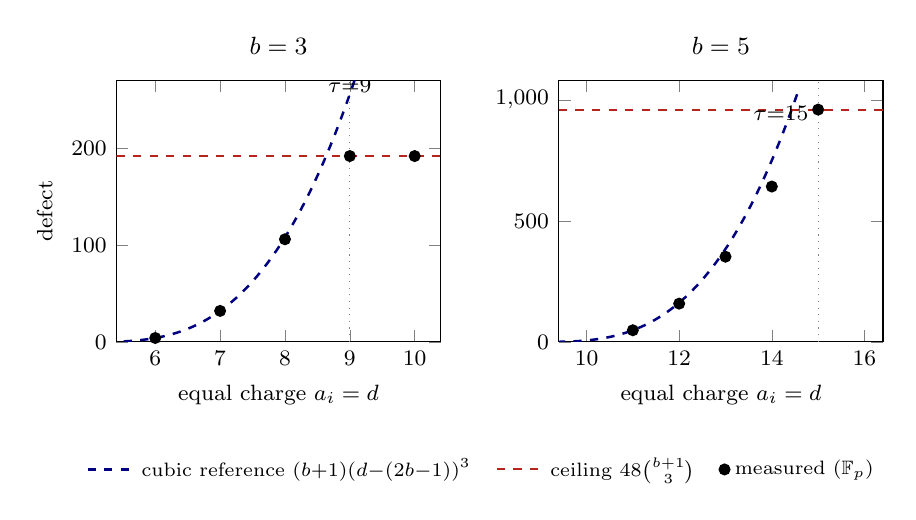
\begin{tikzpicture}
\begin{groupplot}[
  group style={group size=2 by 1, horizontal sep=1.5cm, ylabels at=edge left},
  width=5.7cm, height=4.9cm,
  xlabel={equal charge $a_i=d$}, ylabel={defect},
  ylabel near ticks, xlabel near ticks,
  tick label style={font=\footnotesize}, label style={font=\footnotesize},
  title style={font=\small},
  legend style={font=\scriptsize, draw=none, fill=none, at={(1.13,-0.40)}, anchor=north, legend columns=-1, /tikz/every even column/.append style={column sep=7pt}, cells={align=left}},
  every axis plot/.append style={line width=0.9pt},
]
\nextgroupplot[title={$b=3$}, xmin=5.4, xmax=10.4, ymin=0, ymax=270, xtick={6,7,8,9,10}]
  \addplot[domain=5:9.2, samples=80, dashed, NavyBlue] {4*(x-5)^3};
  \addlegendentry{cubic reference $(b{+}1)(d{-}(2b{-}1))^3$}
  \addplot[BrickRed, dashed, line width=0.7pt] coordinates {(5.4,192) (10.4,192)};
  \addlegendentry{ceiling $48\binom{b+1}{3}$}
  \addplot[only marks, mark=*, mark size=1.7pt, black] coordinates {(6,4) (7,32) (8,106) (9,192) (10,192)};
  \addlegendentry{measured ($\mathbb{F}_p$)}
  \draw[gray, dotted] (axis cs:9,0) -- (axis cs:9,270);
  \node[font=\footnotesize, anchor=south] at (axis cs:9,248) {$\tau{=}9$};
\nextgroupplot[title={$b=5$}, xmin=9.4, xmax=16.4, ymin=0, ymax=1080, xtick={10,12,14,16}, xticklabel style={font=\footnotesize}]
  \addplot[domain=9:14.55, samples=90, dashed, NavyBlue] {6*(x-9)^3};
  \addplot[BrickRed, dashed, line width=0.7pt] coordinates {(9.4,960) (16.4,960)};
  \addplot[only marks, mark=*, mark size=1.7pt, black] coordinates {(11,48) (12,158) (13,352) (14,642) (15,960)};
  \draw[gray, dotted] (axis cs:15,0) -- (axis cs:15,1080);
  \node[font=\footnotesize, anchor=south east] at (axis cs:15,875) {$\tau{=}15$};
\end{groupplot}
\end{tikzpicture}
\caption{The two regimes of the deep-region defect, with measured values from exact $\mathbb{F}_p$ rank computation (filled markers). In these two low-$b$ cases the corrected equal-charge threshold $\rho(b)$ agrees with the cubic-crossing value $\tau(b)$: $\rho(3)=\tau(3)=9$ and $\rho(5)=\tau(5)=15$. Below that point the defect is the $C_b+E-F$ branch of Theorem~\ref{thm:general-toeplitz-saturation}; at and above it the defect is the ceiling $48\binom{b+1}{3}$. All plotted values are reproducible from the accompanying repository.}
\label{fig:ladders}
\end{figure}

\begin{figure}[t]
\centering
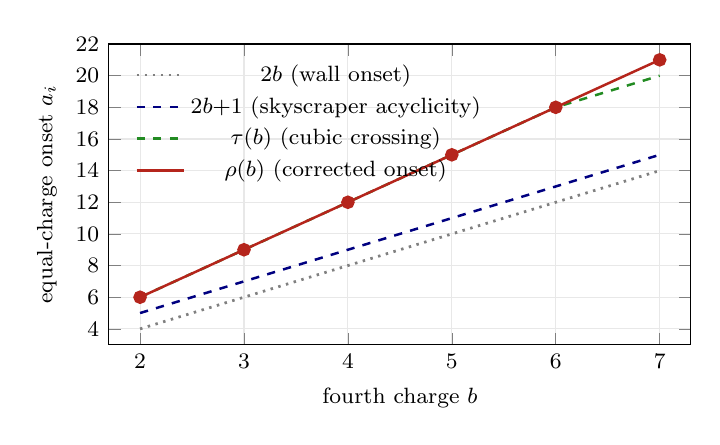
\begin{tikzpicture}
\begin{axis}[
  width=0.74\linewidth, height=5.4cm,
  xlabel={fourth charge $b$}, ylabel={equal-charge onset $a_i$},
  xmin=1.7, xmax=7.3, ymin=3, ymax=22,
  xtick={2,3,4,5,6,7}, ytick={4,6,8,10,12,14,16,18,20,22},
  tick label style={font=\footnotesize}, label style={font=\footnotesize},
  legend style={font=\footnotesize, at={(0.03,0.97)}, anchor=north west, draw=none, fill=none},
  every axis plot/.append style={line width=0.9pt},
  grid=major, grid style={gray!18},
]
  \addplot[gray, dotted, line width=1pt] coordinates {(2,4)(3,6)(4,8)(5,10)(6,12)(7,14)};
  \addlegendentry{$2b$ (wall onset)}
  \addplot[NavyBlue, dashed] coordinates {(2,5)(3,7)(4,9)(5,11)(6,13)(7,15)};
  \addlegendentry{$2b{+}1$ (skyscraper acyclicity)}
  \addplot[ForestGreen, dashed] coordinates {(2,6)(3,9)(4,12)(5,15)(6,18)(7,20)};
  \addlegendentry{$\tau(b)$ (cubic crossing)}
  \addplot[BrickRed, line width=0.9pt] coordinates {(2,6)(3,9)(4,12)(5,15)(6,18)(7,21)};
  \addlegendentry{$\rho(b)$ (corrected onset)}
  \addplot[BrickRed, only marks, mark=*, mark size=2pt] coordinates {(2,6)(3,9)(4,12)(5,15)(6,18)(7,21)};
\end{axis}
\end{tikzpicture}
\caption{Corrected equal-charge saturation onset. The old cubic-crossing reference $\tau(b)=(2b-1)+\lceil2(b(b-1))^{1/3}\rceil$ agrees with the corrected threshold $\rho(b)$ through $b=6$, but fails at $b=7$: $\tau(7)=20$ while $\rho(7)=21$. The corrected threshold is the first $d\ge2b+1$ satisfying $(b+1)(d-1)^3\ge(b-1)(d+1)^3$.}
\label{fig:onset}
\end{figure}

\FloatBarrier
\section{Cross-manifold reproduction: the bicubic}\label{sec:bicubic}

On the bicubic $[\,\PP^2\,\PP^2\,\|\,(3,3)\,]$ the analogous contraction produces a linear system of plane cubics on $\PP^2$. Testing $\mu_V: V\otimes H^0(\PP^2,\cO(e))\to H^0(\PP^2,\cO(e+3))$, $V\subset H^0(\cO(3))$:
for a \textbf{pencil} ($\dim V=2$, base locus $=$ complete intersection of two cubics, $9$ points by B\'ezout) the computed defect climbs $1,3,6,9$ and saturates at $9$ --- the base-locus length; for \textbf{nets and larger} ($\dim V\ge 3$, empty base locus on a surface) the computed defect is $0$ for all $e\ge 4$. This computed bicubic reduction shows the same ceiling-as-intersection-number pattern in a structurally different CICY.

\section{Verification}\label{sec:table}

Predictions in the table below are from~\eqref{eq:rankformula}--\eqref{eq:defectformula} with no fitted parameters; measured ranks are exact finite-field computations by generic-coefficient Gaussian elimination over $\mathbb{F}_p$, $p=2^{31}-1$, with two random sections per point and fixed seed $20260612$.  The finite-field computations certify the stated ranks for the sampled finite-field sections and now serve as reproducibility checks against the characteristic-zero theorem, not as substitutes for its proof.

\begin{center}
\renewcommand{\arraystretch}{1.12}
\begin{tabular}{c c c c c}
\toprule
$(a_1,a_2,a_3)$ & pred.\ rank & meas.\ rank & pred.\ defect & meas.\ defect\\
\midrule
$(4,4,4)$ & $78$ & $78$ & $3$ & $3$\\
$(4,4,5)$ & $102$ & $102$ & $6$ & $6$\\
$(4,4,6)$ & $126$ & $126$ & $9$ & $9$\\
$(4,5,5)$ & $132$ & $132$ & $12$ & $12$\\
$(4,5,6)$ & $162$ & $162$ & $18$ & $18$\\
$(4,6,6)$ & $197$ & $197$ & $28$ & $28$\\
$(4,6,7)$ & $232$ & $232$ & $38$ & $38$\\
$(4,6,8)$ & $267$ & $267$ & $48$ & $48$\\
$(4,7,7)$ & $272$ & $272$ & $48$ & $48$\\
$(4,7,8)$ & $312$ & $312$ & $48$ & $48$\\
$(5,5,5)$ & $168$ & $168$ & $24$ & $24$\\
$(5,5,6)$ & $204$ & $204$ & $36$ & $36$\\
$(5,6,6)$ & $246$ & $246$ & $48$ & $48$\\
$(5,6,7)$ & $288$ & $288$ & $48$ & $48$\\
$(5,6,8)$ & $330$ & $330$ & $48$ & $48$\\
$(5,7,7)$ & $336$ & $336$ & $48$ & $48$\\
$(5,7,8)$ & $384$ & $384$ & $48$ & $48$\\
$(6,6,6)$ & $295$ & $295$ & $48$ & $48$\\
$(6,6,7)$ & $344$ & $344$ & $48$ & $48$\\
$(6,6,8)$ & $393$ & $393$ & $48$ & $48$\\
$(6,7,7)$ & $400$ & $400$ & $48$ & $48$\\
$(7,7,7)$ & $464$ & $464$ & $48$ & $48$\\
\bottomrule
\end{tabular}
\end{center}
\noindent
$22/22$ exact. The full $X$-cohomology satisfies the index identity $\sum_q(-1)^q h^q=2\big(\sum_iD_i+\sum_{i<j<k}D_iD_jD_k\big)$ on every tabulated point, and a $1{,}728$-point sweep over $a\in[4,15]^3$ finds no violation of~\eqref{eq:rankformula}--\eqref{eq:defectformula} and no defect exceeding $48$.

\section{Significance and transferability}\label{sec:significance}

The content of this computation is not the numerical value on a single Calabi--Yau threefold; it is the isolation of a local determinantal source for a cohomology wall. On the tetraquadric the Koszul section map dualises to a contraction $\varphi_s$ whose section-induced Toeplitz local model is computed exactly in Theorem~\ref{thm:general-toeplitz-saturation}. Its maximal-minor ideal is the $(b-1)$st power of the $48$-point base-locus ideal, and its local Buchsbaum--Rim cokernel has length $48\binom{b+1}{3}$. In the acyclic range $a_i\ge2b+1$, this local length converts into the exact global source-target defect formula. The contribution is therefore not a new cohomology formula, since the dimensions in this region are implicit in the systematised formulae of~\cite{ConstantinLukas2019}, but a mechanistic derivation: it explains why a wall of this type occurs, why its height carries the binomial factor, and why the old cubic-crossing threshold must be replaced by the source-target inequality.

The most direct use of such a mechanism is as a check on fitted or learned cohomology formulae. Region-by-region polynomial formulae, including those produced by machine-learning methods that identify the Picard-lattice regions and their polynomials and thereby propose a cohomology formula~\cite{BrodieMLcohomology,ConstantinLukas2019}, are validated against computed dimensions, yet dimensions alone need not determine the underlying law. The present family makes this concrete: the Thom--Porteous count $48\binom{b+1}{3}$ and the factorial pattern $(b+1)!\,2^3$ agree at $b=2$ and $b=3$, at $48$ and $192$, and first diverge at $b=4$, where $480$ separates from $960$, and again at $b=5$, where $960$ separates from $5760$ (Proposition~\ref{thm:decisive}, Remark~\ref{rem:b5}). A formula calibrated only to the agreeing low-charge values cannot distinguish the two before that first divergence; the determinantal mechanism selects the Thom--Porteous candidate in the computed divergent cases. The cohomology dimensions controlled here are moreover of the kind that enter heterotic spectrum computations on this geometry, the tetraquadric being a standard line-bundle model-building space~\cite{BCL2014}, so the mechanism bears on the interpretability of those computations while making no claim about physical spectra. In the general language of algebraic geometry the wall is a jumping locus realised as the degeneracy locus of a bundle map, its height the length of a determinantal thickening of the base locus (Figure~\ref{fig:mechanism}); the same local model is expected to govern other complete-intersection families whenever the Koszul connecting map reduces locally to the same Buchsbaum--Rim format, a transfer we treat as a program rather than an established consequence. The bicubic reduction of Section~\ref{sec:bicubic} is one instance of that mechanism on a structurally different manifold.

\section{Scope, and what is open}\label{sec:open}

The results occupy three levels. The rank formula (Theorem~\ref{thm:rank}) and the saturation ceiling at $48$ (Theorem~\ref{thm:ceiling}) are proved for $b=2$ by two independent arguments, identifying the defect with the degree of the base-locus scheme and the third finite difference of the Koszul Hilbert function. The piecewise region formulae whose values this analysis explains are due to Constantin--Lukas~\cite{ConstantinLukas2019}; the present contribution is a mechanistic account of one wall family, not a new cohomology formula.

For $b\ge3$, Theorem~\ref{thm:general-toeplitz-saturation} proves the Toeplitz determinantal mechanism and gives the exact global defect formula in the acyclic range. The exact finite-field rank computations at $b=3,4,5$ now serve as reproducibility checks and as a numerical distinction from the factorial alternative, not as the mathematical proof.

The former universal threshold $a_i\ge\tau(b)$ is false from $b=7$. The corrected equal-charge threshold is $\rho(b)$ from Corollary~\ref{cor:rho}, and the general multicharge ceiling condition is $(b+1)\prod_i(a_i-1)\ge(b-1)\prod_i(a_i+1)$ together with $a_i\ge2b+1$. What remains open is transferability: whether analogous Toeplitz or Buchsbaum--Rim mechanisms govern higher-codimension complete intersections or sign patterns other than the $3{+}1$ family.

\paragraph{Reproducibility.} All rank determinations are exact finite-field linear algebra; no floating point enters. The verification scripts (the rank verifier, the $1{,}728$-point sweep, the Thom--Porteous evaluation, and this table as CSV) are included with this note's source repository; see the accompanying \texttt{README} for runtimes and expected outputs.

\paragraph{Status of claims.}
\Proven: Prop.~\ref{prop:reduction}, Props.~\ref{prop:dichotomy}(1)--(3), Lemma~\ref{lem:slices}, Theorem~\ref{thm:rank}, Theorem~\ref{thm:ceiling}, Remarks~\ref{rem:minflip}--\ref{rem:why48}, Theorem~\ref{thm:general-toeplitz-saturation}, and Corollary~\ref{cor:rho}.\quad
\Computed: the $b$-law~\eqref{eq:blaw}, the bicubic reproduction, the table, the $b=3$ ceiling by exact $\mathbb{F}_p$ rank, the $b=4$ ceiling at three primes and the $b=5$ ceiling at two primes (the $b=2$ ceiling is \Proven, Theorem~\ref{thm:ceiling}), the low-$b$ coincidence $\rho(b)=\tau(b)$ for $b=2,3,4,5$, with $\rho(b)$ the corrected source-target threshold, and the $b=7$ randomized sparse finite-field confirmation of Remark~\ref{rem:b7sparse} (the dense deterministic $b=7$ rank remains pending).\quad
\Open: multi-equation CICYs; non-$3{+}1$ sign patterns beyond $2{+}2$; the interior $b$-law proof for $b\ge3$ outside the acyclic Toeplitz-saturation range; and transfer criteria for the same Buchsbaum--Rim local model on other complete intersections.

\section*{Code and data availability}
All rank computations in this note are exact finite-field linear algebra; no floating-point arithmetic enters. The rank formula, the $1{,}728$-point sweep, the Thom--Porteous evaluation, and the data underlying Figures~\ref{fig:ladders}--\ref{fig:onset} are reproducible from the accompanying repository; see the \texttt{README} for commands and expected runtimes. The decisive $b=4$ and $b=5$ computations require \texttt{python-flint} and are the computationally heavy steps. The $b=7$ dense deterministic run remains pending; the randomized sparse Wiedemann--Kaltofen--Saunders computation, validated against archived dense $b=3$--$5$ ranks and repeated at independent primes, confirms the predicted defects (Remark~\ref{rem:b7sparse}) and requires no special-memory host.

\begin{thebibliography}{9}
\bibitem{BCL2014} E.~Buchbinder, A.~Constantin, A.~Lukas,
\emph{The moduli space of heterotic line bundle models: a case study for the tetra-quadric},
JHEP \textbf{03} (2014) 025, arXiv:1311.1941, \href{https://doi.org/10.1007/JHEP03(2014)025}{doi:10.1007/JHEP03(2014)025}.
\bibitem{ConstantinLukas2019} A.~Constantin, A.~Lukas,
\emph{Formulae for line bundle cohomology on Calabi--Yau threefolds},
Fortsch.\ Phys.\ \textbf{67} (2019) 1900084, arXiv:1808.09992, \href{https://doi.org/10.1002/prop.201900084}{doi:10.1002/prop.201900084}.
\bibitem{BrodieMLcohomology} C.~R.~Brodie, A.~Constantin, R.~Deen, A.~Lukas,
\emph{Machine learning line bundle cohomology},
Fortsch.\ Phys.\ \textbf{68} (2020) no.~1, 1900087, arXiv:1906.08730, \href{https://doi.org/10.1002/prop.201900087}{doi:10.1002/prop.201900087}.
\bibitem{cohomCalg} R.~Blumenhagen, B.~Jurke, T.~Rahn, H.~Roschy,
\emph{Cohomology of line bundles: a computational algorithm},
J.\ Math.\ Phys.\ \textbf{51} (2010) 103525, arXiv:1003.5217, \href{https://doi.org/10.1063/1.3501132}{doi:10.1063/1.3501132}.
\bibitem{BCDL2020} C.~R.~Brodie, A.~Constantin, R.~Deen, A.~Lukas,
\emph{Index formulae for line bundle cohomology on complex surfaces},
Fortsch.\ Phys.\ \textbf{68} (2020) no.~2, 1900086, arXiv:1906.08769, \href{https://doi.org/10.1002/prop.201900086}{doi:10.1002/prop.201900086}.
\bibitem{BC2020} C.~R.~Brodie, A.~Constantin,
\emph{Cohomology chambers on complex surfaces and elliptically fibered Calabi--Yau three-folds},
arXiv:2009.01275, \href{https://doi.org/10.48550/arXiv.2009.01275}{doi:10.48550/arXiv.2009.01275}.
\bibitem{Eisenbud} D.~Eisenbud, \emph{Commutative Algebra with a View Toward Algebraic Geometry}, Springer GTM 150 (1995).
\bibitem{Hartshorne} R.~Hartshorne, \emph{Algebraic Geometry}, Springer GTM 52 (1977).
\end{thebibliography}

\end{document}
